	\section{Computação nas Nuvens}
Inicialmente acreditava-se que a melhor forma de conseguir poder de processamento adequado para empresas de grande porte ou universidade era apenas por meio de grandes, robustos e caros mainframes. Entretanto, com o passar dos anos percebeu-se que adicionando vários computadores mais simples, trabalhando em conjunto, era possível obter os mesmo resultados alcançados com a utilização do caro e de difícil manutenção mainframe.
A partir dessa ideia, surgiu o conceito de cluster, no qual vários computadores idênticos são interligados fisicamente por meio de uma rede, com a proposta de trabalharem como se fossem apenas uma só máquina \cite{buyya1}. \\

Em seguida, essa ideia evoluiu para o conceito de grid, o qual é um tipo de sistema paralelo e distribuído que possibilita, dinamicamente, o compartilhamento, a seleção, e a agregação de recursos 'autônomos', geograficamente distribuídos, dependendo de sua disponibilidade, capacidade, desempenho, custo e requisitos de qualidade de serviço dos usuários \cite{buyya1}. Isso proporcionou que várias instituições (principalmente as universidades) compartilhassem o poder de processamento do grid. \\

Assim, diante de uma constante evolução nessa área, surgiu, nos anos 2000, a ideia de computação em nuvens, na qual vários computadores, notebooks ou até mesmo mainframes são conectados via rede, de forma a trabalharem como se fossem uma só máquina, porém com a diferença de que qualquer pessoa pode usar seu computador pessoal para se conectar a nuvem, e utilizar o poder de processamento e/ou armazenamento da nuvem desde que seja autorizada. Como o conceito de computação em nuvens foi criado pelo mercado (diferente do grid que foi desenvolvido em meio acadêmico) é natural que a concessão de autorização para utilizar seus serviços seja por meio da forma de pagamento em dinheiro. \\

A indústria disponibiliza diferentes modelos de nuvem para conquistar distintos modos de demandas que seus consumidores possam ter, as mais comuns são a Infraestrutura como Serviço (IaaS), a Plataformas como Serviço (PaaS) e o Software como Serviço (SaaS). Porém, devido a sua natureza econômica, a computação em nuvem precisou criar conceitos próprios, como é o caso do conceito referente ao Acordo de Nível de Serviço (SLA), no qual o cliente e o fornecedor da nuvem assinam um contrato formalizando as responsabilidades de cada um; ou a Qualidade de Serviço (QoS) a qual metrifica se o acordo do SLA está sendo cumprido adequadamente \cite{buyya2}. \\

Tendo em mente o mesmo principio que levou a criação do paradigma da computação em nuvens, percebeu-se que apesar de sua proposta inicial passar a sensação de que os recursos computacionais da nuvem são ilimitados, na verdade eles são finitos. Desta forma, sentiu-se a necessidade de expandir o conceito de nuvem, e assim surgiu o conceito de Federação de Nuvens (ou inter-nuvem), o qual é de forma simplificada, uma grande nuvem formada por outras nuvens. Logo, nuvens sobrecarregadas podem transferir tarefas para nuvens com recursos suficientes para satisfazer a demanda, aumentando assim a sensação para o consumidor final de que os recursos da nuvem são ilimitados. \\

\begin{figure}[htb]
	\begin{center}
		
		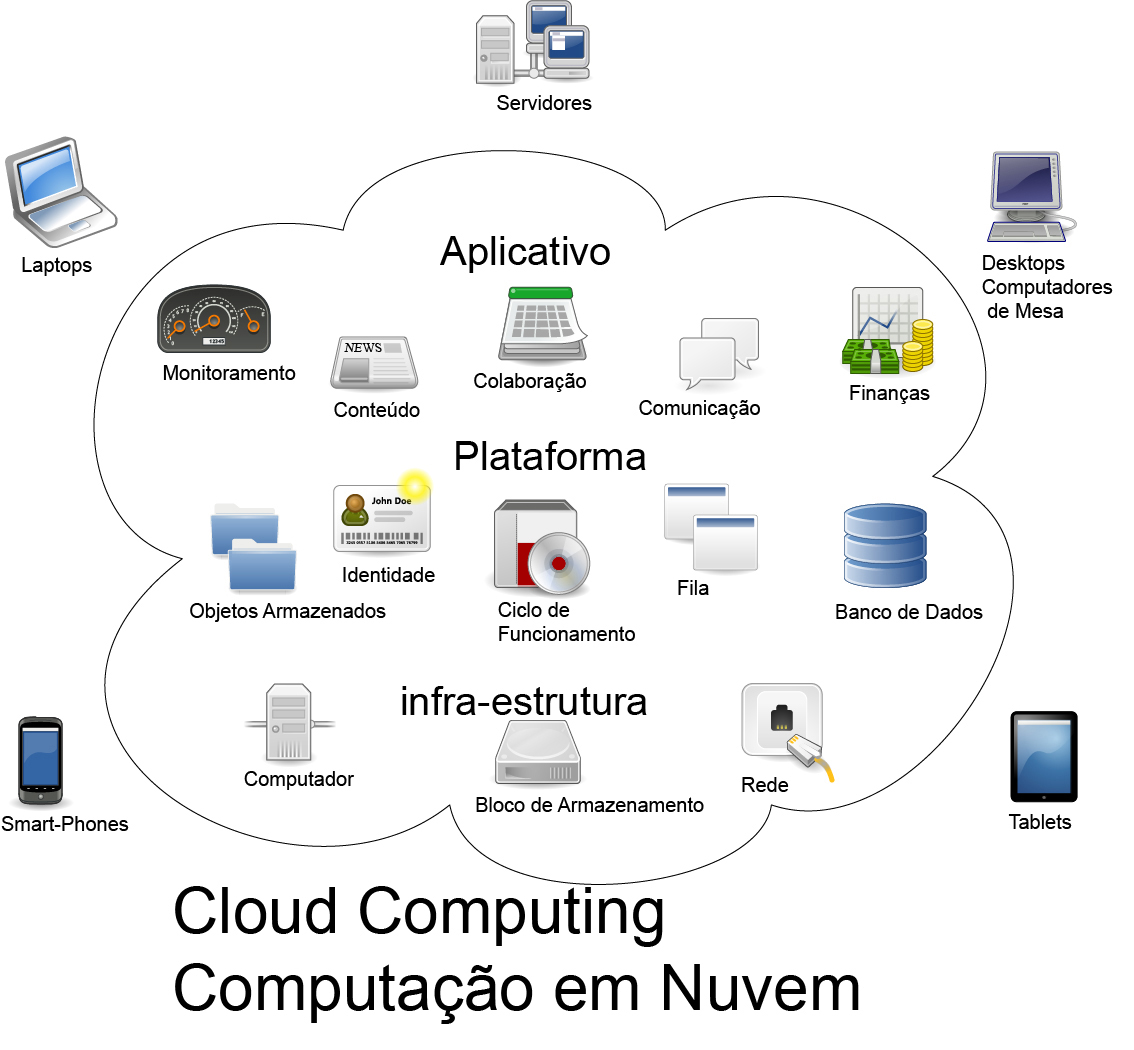
\includegraphics[clip,width=10.0cm]{images/image3.jpg}
		\caption{Visão geral da Computação na Nuvem}
		\label{fig:vis_sis}
	\end{center}
\end{figure}

Como o conceito de computação nas nuvens é relativamente recente, ainda há muitos desafios a serem superados, algoritmos a serem aprimorados, arquiteturas definidas e abordagens testadas. Do ponto de vista deste trabalho, o desafio abordado é sobre o desenvolvimento de um sistema de arquivos funcional, seguro e eficiente. Visto que o fato de a nuvem tratar-se essencialmente de um robusto sistema distribuído, como e onde armazenar os mais variados arquivos de todos os seus usuários de forma segura (tanto do ponto de vista que os dados não serão perdidos e nem acessados por usuários não autorizados) não é uma tarefa trivial. Bessani et al em \cite{bessani1} apresenta o SCFS, o qual é um sistema de arquivos projetado para trabalhar especialmente em ambientes de nuvens federadas (cloud-of-clouds) que possui algumas características interessantes que podem ser estendidas para a maioria dos sistemas de arquivos ditribuidos, tais propriedades são listadas logo abaixo. \\

\begin{itemize}
	\item Sempre escreva, evite leituras\\
	Visto que em ambientes de computação na nuvens, escrever é tipicamente mais barato (no sentido monetário, não de processamento) do que ler, o SCFS atualizar os arquivos na nuvem com frequência, entretanto, sempre que possível tentar manter cópias locais dos aquivos no computador do usuário para evitar leituras. Isto é comprovado pelo fato de que os provedores de nuvem tendem a deixar o upload de dados gratuito, cobrando apenas pelo download como forma de atrair mais clientes.
	\item Espaço de Nomes Privados (Private Name Spaces ou PNS)\\
	PNS é uma nova estrutura de dados local utilizada para armazenar a informação dos metadados referentes aos vários arquivos, que não podem ser compartilhados entre diferentes usuários, como um objeto único guardado na nuvem contendo todos metadados privados do usuário.
	\item Múltiplas nuvens redundantes\\
	Os arquivos são salvos em várias nuvens diferentes para assim aumentar drasticamente a tolerância à falhas contra arquivos corrompidos, perda de arquivos ou nuvens temporariamente fora do ar no momento em que algum arquivo armazenado nela deve ser retornado. Porém, isto levanta o problema de garantir que todas as várias copias rudantes dos arquivos sejam acessadas apenas por usuários autorizados, este problema é solucionado ao fazer com que todos os arquivos armazenados na nuvem sejam criptografados.
\end{itemize}


\subsection{As necessidades da Computação nas Nuvens}
Os fornecedores responsáveis pela nuvem estão sempre interessados em aumentar o lucro gerado, para tal eles tendem a ofertar a maior variedade possível de serviços para suportar os mais diversificados tipos de serviços. Este tipo de abordagem possui um custo, pois é necessário levar em consideração todas essas questões políticas no momento de montar a arquitetura adequada para a nuvem, isto inclui os computadores que a formaram, a tecnologia usada, o local físico das instalações e inclusive os softwares que irão gerenciar todo o sistema, nesse conjunto de gerenciadores está incluso o escalonador, o qual será responsável por distribuir adequadamente as tarefas pelos nós da nuvem da forma mais otimizada possível para agilizar a performance sem permitir que nós fiquem sobrecarregados, enquanto outros estão ociosos. Todavia, estas não são escolhas triviais \cite{drasko1}.\\

Quanto maior for a quantidade de usuários utilizando os serviços prestados pela nuvem, maior será a dificuldade de manter todo o sistema em equilíbrio e obedecendo a SLA de cada consumidor, enquanto mantém a QoS em níveis aceitáveis. Visto que para os usuários a nuvem passa a sensação de possuir recursos ilimitados, entretanto eles são obviamente finitos e dependendo da quantidade e dificuldade das requisições, a infraestrutura da nuvem pode não suportar atender a todos sem violar a SLA de alguns (ou vários) consumidores. Isso é um caso desagradável tanto para o provedor quanto para os clientes. Mas o que fazer para manter a QoS elevada mesmo quando a infraestrutura da nuvem está sobrecarregada? A solução mais aceita atualmente é a federação de nuvens (inter-nuvens ou cloud-of-clouds), pois desta forma os provedores de serviço podem manter a SLA de seus clientes intacta “pegando emprestados” recursos computacionais das outras nuvens participantes da federação em momentos de necessidade, sendo que em troca basta “emprestar” seus recursos para outros provedores em momentos que o sistema esteja trabalhando com sobra de recursos, o que é mostrado por Buyya et al em \cite{buyya2} e por Celesti et al em \cite{celesti1}.\\

Outro bom exemplo da necessidade e da adaptabilidade da computação nas nuvens é o controle de desastre que ela oferece. Uma forma em que esse controle pode ser representado é no caso de um datacenter cair o sistema não fica fora do ar, pois todos os dados e processos que estavam armazenados e rodando no datacenter podem ser replicados em outra nuvem. É justamente nesta propriedade que nasce uma questão importantíssima: como os dados são armazenados na nuvem? Como eles são distribuídos? Este trabalho pretende, ao final, mostrar um sistema de arquivos distribuídos que poderia ser facilmente utilizado num ambiente de nuvem federadas quanto em um sistema de arquivos distribuídos local ou em uma grid de forma segura, robusta e garantido o controle de desastre requerido por um sistema de nuvem sério.\\
	
	%texto.... referência \cite{borsley96}